\documentclass[a4paper, 10pt, dvipdfmx]{jlreq}

\usepackage{ascmac}
\usepackage{amsmath,amsfonts,amssymb}
\usepackage{bm}
\usepackage{mathtools}
\usepackage{siunitx}
\usepackage[dvipdfmx]{graphicx}
\usepackage[dvipdfmx]{color}
\usepackage[dvipdfmx, colorlinks=true, allcolors=blue]{hyperref}
\usepackage{listings, jlisting}
\usepackage{tikz}
\usepackage{physics}
\usepackage{url}

\Urlmuskip=0mu plus 10mu
\allowdisplaybreaks[4]
\frenchspacing
\definecolor{OliveGreen}{rgb}{0.0,0.6,0.0}
\definecolor{Orenge}{rgb}{0.89,0.55,0}
\definecolor{SkyBlue}{rgb}{0.28, 0.28, 0.95}
\lstset{
  language={c++},
  basicstyle={\ttfamily},
  identifierstyle={\small},
  ndkeywordstyle={\small},
  frame=single,
  breaklines=true,
  numbers=left,
  xrightmargin=0zw,
  xleftmargin=3zw,
  numberstyle={\scriptsize},
  lineskip=-0.9ex,
  keywordstyle={\small\bfseries\color{SkyBlue}},  
  commentstyle={\color{OliveGreen}}, 
  stringstyle={\small\ttfamily\color{Orenge}}    
}

\begin{document}

\title{2020年度 大問2}
\author{hari64boli64 (hari64boli64@gmail.com)}
\date{\today}
\maketitle


\section{問題}

\begin{align*}
    f(x;\mu)=\frac{1}{\mu}e^{-\frac{x}{\mu}}
\end{align*}

\begin{align*}
    Y_i= \left\{
    \begin{array}{ll}
        a   & (X_i \leq a) \\
        X_i & (X_i > a)
    \end{array}
    \right.
\end{align*}

\section{解答}

\subsection*{(1)}

$Y_1$の期待値は

\begin{align*}
    \int_0^a af(x;\mu)dx + \int_a^\infty xf(x;\mu)dx=a+\mu e^{-\frac{a}{\mu}}
\end{align*}

\subsection*{(2)}

$g(\hat{\mu})-a=\hat{\mu}e^{-\frac{a}{\hat{\mu}}}$を考える。

存在は、連続性と$\lim_{x \to \infty}\hat{\mu}e^{-\frac{a}{\hat{\mu}}} \to \infty$より明らか。

一意性は、微分すると狭義単調と分かるので明らか。

\subsection*{(3)}

自信なし。

まず、$P(M=m)$を求める。

$P(Y_1=a)=\int_0^a{f(x;\mu)}dx=1-e^{-\frac{a}{\mu}}$より、$P(M=m) = {}_NC_m (1-e^{-\frac{a}{\mu}})^m(e^{-\frac{a}{\mu}})^{N-m}$

次に、$P(\overline{Y}\leq b | M=m)$を求める。

\begin{align*}
    P(\overline{Y}\leq b | M=m) & = P\left( \sum_{i=1}^N Y_i \leq Nb \middle| M=m \right)  \\
                                & = P\left( am + \sum_{i=1}^{N-m} (Y_i+a)  \leq Nb \right) \\
                                & = P\left( \sum_{i=1}^{N-m} Y_i  \leq N(b-a) \right)      \\
                                & = \int_0^{N(b-a)} f_{N-m}(y) dy                          \\
                                & = \int_a^{b} Nf_{N-m}(Ny-a) dy                           \\
\end{align*}

ただし、一行目から二行目の変形で、指数分布の無記憶性を用いた。

また、$f_{N-m}$で、指数分布を$N-m$個重ね合わせた分布を示している。

これは、ガンマ分布に従うことが一般に知られている。(後述)

以上より、

\begin{align*}
    P(M=m,\overline{Y}\leq b) & = P(M=m)P(\overline{Y} \leq b|M=m)                                                                                                          \\
                              & = {}_NC_m (1-e^{-\frac{a}{\mu}})^m(e^{-\frac{a}{\mu}})^{N-m} \int_a^{b} N f_{N-m}(Ny-a) dy                                                  \\
                              & = {}_NC_m (1-e^{-\frac{a}{\mu}})^m(e^{-\frac{a}{\mu}})^{N-m} \int_a^{b} \frac{N}{(N-m-1)!\mu^{N-m}} (Ny-a)^{N-m-1} e^{-\frac{Ny-a}{\mu}} dy \\
\end{align*}

\subsection*{(4)}

$\mu$に関連する部分だけ取り出すと、

\begin{align*}
    M(\mu) & = (1-e^{-\frac{a}{\mu}})^m(e^{-\frac{a}{\mu}})^{N-m}  \frac{1}{\mu^{N-m}} e^{-\frac{Ny-a}{\mu}}
\end{align*}

となるが、これを微分するのは大変な困難を伴うように思われる。

なので、別の方針を考える。

\begin{align*}
    h(m,y;\mu) & =\dv{y}\qty(\int_a^y{h(m,y';\mu)}dy')  \\
               & =\dv{y}\qty(P(M=m,\overline{Y}\leq y)) \\
               & =P(M=m,\overline{Y}=y)                 \\
\end{align*}

ただし、最後の変形で、累積分布関数の微分が確率密度関数になることを用いた。

細かい議論は(2)などと同様になるので省くが、無記憶性を用いた議論や適切な変形を経ると、結局のところ、指数分布の確率密度関数$f(x;\mu)$について、ある値$Y$を取る確率が最大になるような$\mu$が、ただ一つ存在することを示す問題に帰着されると思われる。

これは、(2)の議論とほぼ同様である。

以下では、おまけ程度に、上で示した問題の解を与える。

\begin{align*}
    \pdv{\mu}f(Y;\mu) & =-\frac{1}{\mu^2}e^{-\frac{Y}{\mu}}+\frac{1}{\mu}\frac{Y}{\mu^2}e^{-\frac{Y}{\mu}} \\
                      & =\frac{-mu+Y}{\mu^3}e^{-\frac{Y}{\mu}}
\end{align*}

よって、$\pdv{\mu}f(Y;\mu)=0$となる$\mu$は、$Y=\mu$の時、これのみである。

以上で、大まかには題意が示された。

より詳細な議論を、本来は行うべきであろう。

\section{知識}

指数分布は再生性を持たない。つまり、$X_1,X_2,\cdots$が独立に指数分布に従うとしても、$X_1+X_2+\cdots$は指数分布に従わない。これは一般にはアーラン分布に従う。特に、今回はガンマ分布に従う。これは以下の畳み込みの式と帰納法で示せる。

\begin{align*}
    f_{Y(=X_1+X_2)}(y)=\int_0^{y}{f_{X_1}(x)f_{X_2}(y-x)dx}
\end{align*}

同じ指数分布の重ね合わせがガンマ分布になることを示す。

\begin{align*}
    f_1(x;\mu) & =\frac{1}{\mu}e^{-\frac{x}{\mu}}                                                 \\
    f_2(x;\mu) & =\int_0^x{f_1(y;\mu)f_1(x-y;\mu)dy}                                              \\
               & =\int_0^x{\frac{1}{\mu}e^{-\frac{y}{\mu}}\frac{1}{\mu}e^{-\frac{x-y}{\mu}}dy}    \\
               & =\frac{1}{\mu^2}\int_0^x{e^{-\frac{x}{\mu}}dy}                                   \\
               & =\frac{1}{\mu^2}xe^{-\frac{x}{\mu}}                                              \\
    f_3(x;\mu) & =\int_0^x{f_2(y;\mu)f_1(x-y;\mu)dy}                                              \\
               & =\int_0^x{\frac{1}{\mu^2}ye^{-\frac{y}{\mu}}\frac{1}{\mu}e^{-\frac{x-y}{\mu}}dy} \\
               & =\frac{1}{\mu^3}\int_0^x{ye^{-\frac{x}{\mu}}dy}                                  \\
               & =\frac{1}{2\mu^3}x^2e^{-\frac{x}{\mu}}                                           \\
    f_n(x;\mu) & =\int_0^x{f_{n-1}(y;\mu)f_1(x-y;\mu)dy}                                          \\
               & =\frac{1}{(n-1)!\mu^n} x^{n-1} e^{-\frac{x}{\mu}}                                \\
\end{align*}

頑張れば、ガンマ分布の形を覚えていなくても、畳み込み計算から示すことが出来る。

指数分布の無記憶性を示す。

\begin{align*}
    P(X>s+t|X>s) & =\frac{P(X>s+t)}{P(X>s)}                                                                                         \\
                 & =\frac{\int_{s+t}^{\infty}\frac{1}{\mu}e^{-\frac{x}{\mu}}dx}{\int_{s}^{\infty}\frac{1}{\mu}e^{-\frac{x}{\mu}}dx} \\
                 & =\frac{e^{-\frac{s+t}{\mu}}}{e^{-\frac{s}{\mu}}}                                                                 \\
                 & =e^{-\frac{t}{\mu}}                                                                                              \\
                 & =P(X>t)                                                                                                          \\
\end{align*}

\begin{itembox}[l]{\href{https://mathlandscape.com/exp-distrib-memoryless/}{指数分布の無記憶性とその証明}}
    指数分布とは,「コールセンターに次に電話がかかってくるまでにかかる時間」や「電化製品が次に壊れるまでの時間」などに用いられます。「昨日コールセンターに電話がかかってきたから,今日はかかってこないだろう」とか「昨日電化製品が壊れなかったから,今日は壊れないだろう」とか,そういうことはないわけですから,この事象には,無記憶性があるといえるわけですね。
\end{itembox}

そして、最後の(4)などは、図\ref{img:param}が念頭にあると、より分かりやすいと思われる。

とある$x$でこのグラフを切った時に、最大の値を取るような$\lambda$は、ただ一つだけというのが、この問題の視覚的な理解であると思われる。

\newpage

\begin{figure}[htbp]
    \begin{center}
        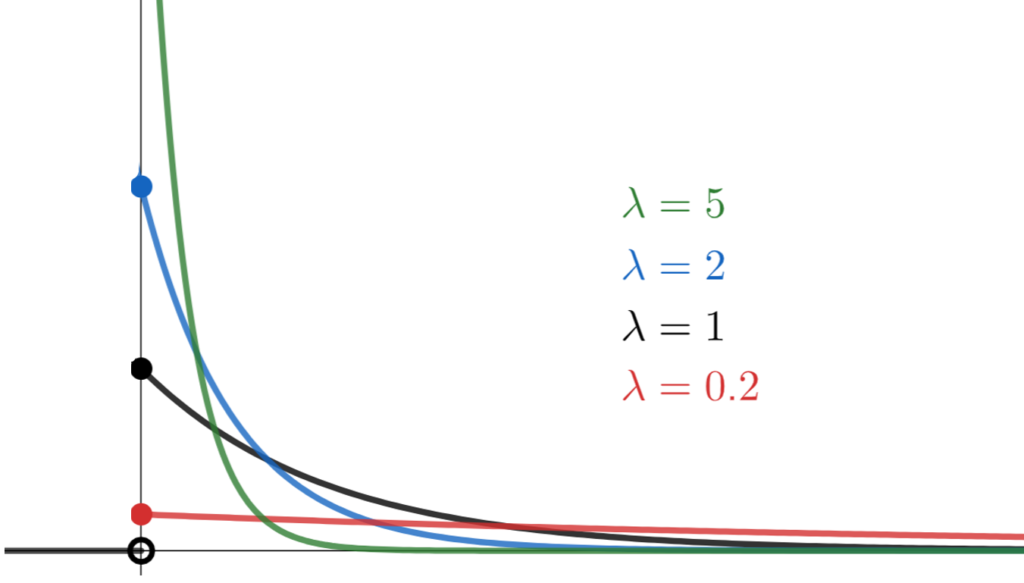
\includegraphics[height=80mm]{exp-distrib-many-1024x583.png}
        \caption{パラメータ毎の指数分布 \cite{site:1}}
        \label{img:param}
    \end{center}
\end{figure}


\begin{thebibliography}{9}
    \bibitem{site:1}
    数学の景色.“指数分布の定義と例と性質まとめ”.2022年3月6日.\url{https://mathlandscape.com/exp-distrib/}
    \bibitem{site:2}
    数学の景色."指数分布の無記憶性とその証明".2021年9月23日.\url{https://mathlandscape.com/exp-distrib-memoryless/}
\end{thebibliography}

\end{document}
